% !TEX encoding = UTF-8 Unicode
% !TEX TS-program = xelatex

\documentclass{article}
	\usepackage{fontspec}
	\usepackage{tikz}
	\usepackage{listings}
\begin{document}



	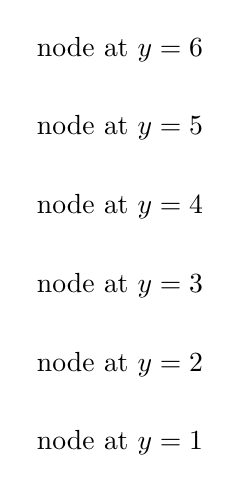
\begin{tikzpicture}
		\foreach \y in {1, 2, 3, 4, 5, 6}{
			\node at (0, \y) {node at $y = \y$};
		}
	\end{tikzpicture}



\lstset{language=[latex]tex,tabsize=4}
\lstset{moretexcs={draw}}
\fontspec{SourceCodePro-Regular}



%%%%%%%%%%%%%%%%%%
\begin{lstlisting}
% !TEX encoding = UTF-8 Unicode
% !TEX TS-program = pdflatex
\documentclass{article}
	\usepackage{tikz}
\begin{document}
	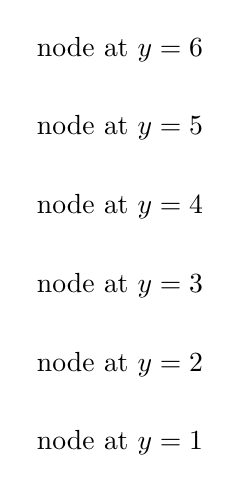
\begin{tikzpicture}
		\foreach \y in {1, 2, 3, 4, 5, 6}{
			\node at (0, \y) {node at $y = \y$};
		}
	\end{tikzpicture}
\end{document}
\end{lstlisting}
%%%%%%%%%%%%%%%%



\end{document}